\section{Problem Exploration}
\label{sec:problem-exp}
Before starting the development process the problem domain has to be explored to figure out what the focus of the project should be. For this we utilized the ESSENCE innovation methodology. The result was two prototype configurations described in the following sections.

\subsection{Run Together}
For the first prototype configuration the challenge was formulated as "How can we motivate people to exercise?". This is based in the problem domain of declining activity levels for people in Western societies. More and more jobs are highly sedentary and this poses an elevated health risk. 
\vspace{10pt}

\subsubsection{Paradigm}
The use context for this application would be a person wanting to increase their fitness by running. The application developed should motivate people to exercise via social interaction and help them see their progress.
\vspace{10pt}

The stakeholders in this project are people who want help motivating themselves to exercise and who would like to exercise in a social setting. The main focus is on the social aspect of exercising. 
\vspace{10pt}

The user scenario is as follows: the user decides to go for a run. They open up the application, choose a route and invite their friends to go out running with them. All friends can respond to the invitation and join in the running. Once the run is over the user can review the log of the route (distance, time etc) and compare it to previous runs.  

\subsubsection{Product}
For this application several afforddances exist. For example the widespread use of smartphones in today's society means that it is safe to assume that a user will have a large amount of friends with smartphones that can download the application and add each other to their friends lists. Both \ac{GPS} and accelerometer are built-in features in virtually all existing smartphones and these enable precise tracking of distance and speed. The vibrator and loudspeakers in a smartphone allow for both tactile and audio feedback to communicate with the user without them looking at their screen. With mobile networks covering more and more of the world constant Internet connectivity also means that a user can interact with their friends while running.
\vspace{10pt}

The design of the product should be a smatphone application and a central server storing important data such as profiles, friends lists, training logs etc.
\vspace{10pt}

The components of the product are
\begin{itemize}
\item A personal profile with friends list, personal records and a list of saved routes.
\item An Internet connection to friends' devices.
\item Smartphone features such a \ac{GPS} for tracking during the run.
\end{itemize}

\subsubsection{Project}
The vision of the project is expressed in a metaphor: a running club. The application should use the feedback and tracking options provided by the smartphone to give the user a feeling of running with their friends, even if said friends are not physically present during the run. 
\vspace{10pt}

The vision can also be expressed in a vision pattern, illustrated in \autoref{fig:visionpattern1}

\begin{figure}[ht]
\begin{center}
 \caption{Vision Pattern}
 \label{fig:visionpattern1}
 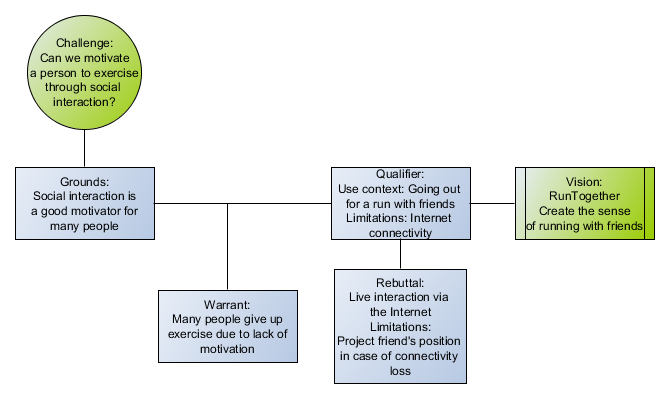
\includegraphics[scale=0.5]{img/visionpattern1.png}
\end{center}
\end{figure}
\vspace{10pt}

The core features of the application would be 
\begin{itemize}
\item Audio and tactile feedback on your running partners' positions
\item Arbitrary number of running partners
\item Visualization of your partners relative to your route (i.e. where would they be on your route if they were running with you).
\item Tracking of run to compare with previous exercise logs.
\item Connection to friends during the run
\end{itemize}

\subsubsection{Process}
To facilitate convergent thinking about the project the focus was on creating value for the user through social interaction. 
\vspace{10pt}

The idea of virtually running with a number of friends was evaluated with a \ac{SWOT} analysis show in \autoref{tab:SWOT1}

\begin{figure}[ht]
 \caption{SWOT analysis}
 \label{tab:SWOT1}
 \begin{tabular}{| l | l |}
 \hline
Strength & Weaknesses \\ 
Social interaction is good motivation & Requires friends to have smartphones \\
Spontaneous exercise through & Friends must also be interested \\
invitations from friends &  in fitness \\
 & Requires stable Internet connection \\ \hline
Opportunities & Threats \\ 
Social fitness network & Unstable Internet \\
 & Cheating friends could ruin the fun \\
 & Running with friends might lose its \\
 & appeal after a while \\
\hline
 \end{tabular}
\end{figure}
\vspace{10pt}

The findings of the analysis as well as subsequent discussion of the idea led to the conclusion that the social aspect with friends is already heavily utilized in existing applications and so the idea is not novel. Running with friends could lose its appeal for some people because the novelty relies on a large circle of friends who have the app installed. It is not necessarily the best way to go about motivating very competitive people for example. It is also easy to "cheat" for a competitive person with poor ethics to always end up as the "winner" of the run, even if there is no explicit competition.

\subsection{RunOff}
For the second prototype we shifted the challenge to "Can we motivate people to exercise and keep exercising?". Many people start to exercise but then lose interest and keeping it up is vital to enjoying it and making it a habit. 

\subsubsection{Paradigm}
The paradigm for this prototype is pretty much the same as the previous prototype, however the stakeholder are somewhat different. For this prototype the stakeholders are a subset of people who want to increase their fitness, namely the ones who are competitive and can utilize this as their primary motivation. 
\vspace{10pt}

The scenario for this prototype is a person who wants to go for a run. They choose a route and find a random match of equal skill online. They race against this person and the server finds a winner. After the run the user can review a log of the run and compare it to previous runs as well as see their ranking on a leaderboard. 

\subsubsection{Product}
The affordances are the same and so is the design, except for this prototype, competitive as it is, it's important that the server has anti-cheat measures to prevent people from cheating their way up the leaderboard.
\vspace{10pt}

The components of the product are the same, except with the new focus on competition a core part of the product is that a person now has a ranking to ensure that they are matched against a fair opponent and to place them on the leaderboard.
\vspace{10pt}

The architecture of the product is seen in

\begin{figure}[ht]
\begin{center}
 \caption{Architecture}
 \label{fig:architecture}
 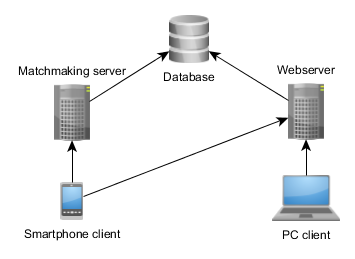
\includegraphics[scale=0.75]{img/architecture.png}
\end{center}
\end{figure}

\subsubsection{Project}
The metaphor expressing the core vision of this prototype is a championship. The user should feel like they are racing against an opponent, pushing themselves to reach the finish line first. The feedback of options in a smartphone should be utilized to give the user a feeling of excitement during the run.

The vision is expressed in the vision pattern in \autoref{fig:visionpattern2}

\begin{figure}[ht]
\begin{center}
 \caption{Vision Pattern}
 \label{fig:visionpattern2}
 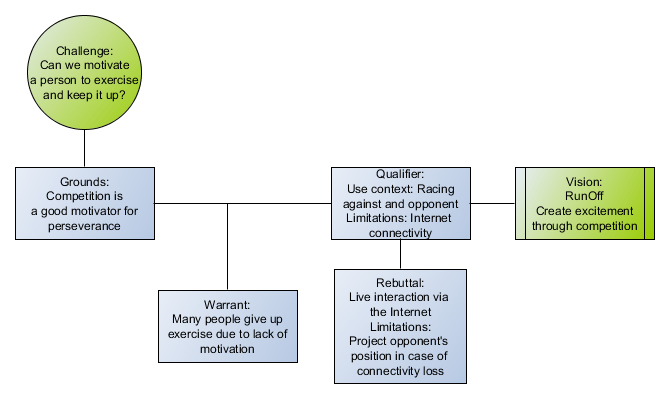
\includegraphics[scale=0.5]{img/visionpattern2.png}
\end{center}
\end{figure}

The group also wrote an elevator pitch for the vision, seen in \autoref{fig:elevatorpitch}

\begin{figure}[ht]
\begin{center}
 \caption{Elevator Pitch}
 \label{fig:elevatorpitch}
 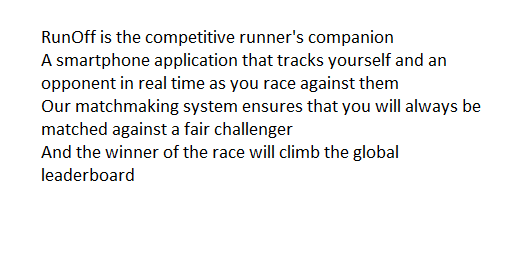
\includegraphics[scale=0.5]{img/elevatorpitch.png}
\end{center}
\end{figure}
\vspace{10pt}

The features of the product are the same as for the previous prototype, however the anti-cheat measure are important to help the user trust the rankings.

\subsubsection{Process}
Agains the focus was on creating value for the user, however instead of doing it through friendly social interaction it is done through competition. 
\vspace{10pt}

The idea of running against a stranger of roughly equal skill as motivation to exercise was evaluated through a \ac{SWOT} analysis, shown in \autoref{tab:SWOT2}

\begin{figure}[ht]
 \caption{SWOT analysis}
 \label{tab:SWOT2}
 \begin{tabular}{| l | l |}
 \hline
Strength & Weaknesses \\ 
Competition works as good motivation & Unstable Internet connections \\ 
Ranking gives a sense of achievement & Non-competitive users are put off \\
Fair competition & \\ \hline
Opportunities & Threats \\ 
Expand with social network & Unstable Internet \\
 & Cheating \\
\hline
 \end{tabular}
\end{figure}
\vspace{10pt}

Through the evaluation and discussion it became clear that this idea was more novel than the previous. The idea of social interaction during the activity and real-time competition are new compared to the known existing solutions. Having a leaderboard to climb as well as people to compete against no matter how many friends you have is very motivating, however it is very important that cheating is prevented because distrust of the leaderboard from the users would completely destroy the idea.

The difference between the two prototypes are highlighted in \autoref{fig:prototypeconfig1} and \autoref{fig:prototypeconfig2}

\begin{figure}[ht!]
\begin{center}
 \label{fig:prototypeconfig1}
 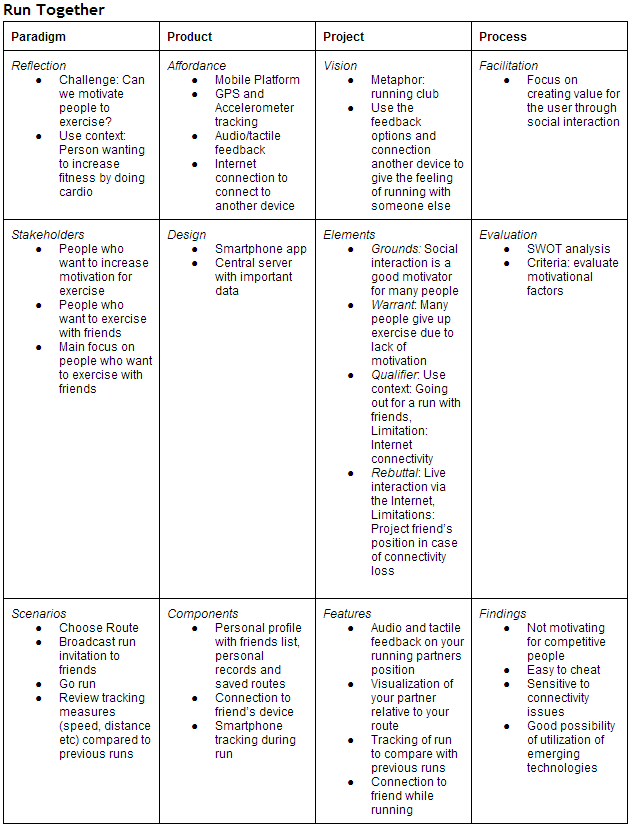
\includegraphics[width=\textwidth]{img/prototypeconfig1.png}
 \caption{Prototype Configuration 1}
\end{center}
\end{figure}

\begin{figure}[ht!]
\begin{center}
 \label{fig:prototypeconfig2}
 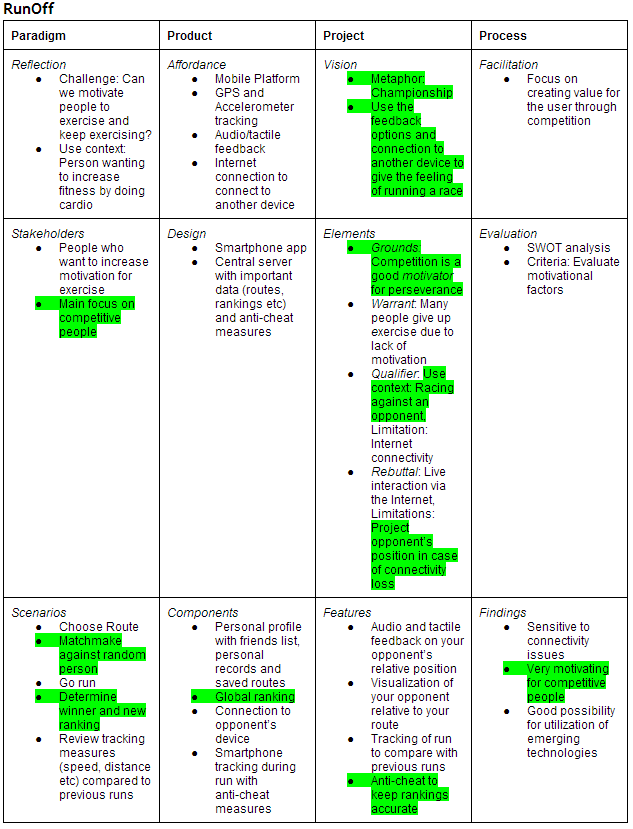
\includegraphics[width=\textwidth]{img/prototypeconfig2.png}
 \caption{Prototype Configuration 2}
\end{center}
\end{figure}